\documentclass[a4paper,,12pt]{abntex2}
\usepackage[Portuguese]{babel}
\usepackage[utf8]{inputenc}
\usepackage[T1]{fontenc} 
\usepackage{fancyhdr} 
\usepackage{amsfonts}
\usepackage{amssymb}
\usepackage{amsmath}
\usepackage{graphicx}
\author{Gabriel R. Munhoz}
\title{Propriedades Coligativas}

\begin{document}
\maketitle
\section{Abaixamento da pressão de vapor}

Um líquido em um sistema fechado sempre entrará em equilíbrio com seu vapor, e este sempre aplicará uma certa pressão sobre o líquido. Essa pressão se muito pequena classifica o mesmo como sendo não-volátil e se grande o caracteriza como sendo volátil.

A adição de soluto não-volátil e não-eletrólito faz com que a pressão de vapor diminua e isso ocorre de acordo com a concentração do soluto e não com o tipo de partícula. A causa dessa interferência pode ser explicada devido a ocupação de parte da superfície do líquido pelo soluto, assim o líquido tem mais dificuldade em se transformar em vapor, com isso a pressão de vapor é menor (Figura 1).

\begin{figure}[!htp]
\centering
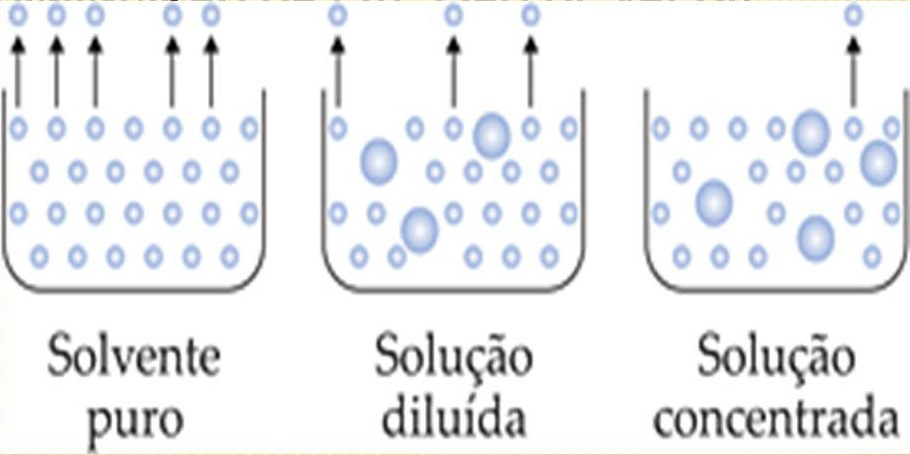
\includegraphics[scale=0.5]{../slide_10.jpg}  
\caption{Diferença entre líquido puro e soluções quanto a pressão de vapor}
\end{figure}

\section{Diminuição do ponto de congelamento}

Devido à variação da pressão de vapor ocasionada pela adição de um soluto não-volátil o ponto de congelamento de um liquido puro é mais alto do que em uma solução. E isso acontece por causa da dificuldade que a solução possui para aumentar sua pressão de vapor.

E este fato é muito utilizado no cotidiano dos países que fazem muito frio, pois ao adicionarem sal na neve das estradas, por exemplo, ela acaba derretendo e diminuindo o número de acidentes, além de utilizam um composto no combustível dos carros também para que ela não congele tão facilmente quando as temperaturas se encontram muito baixas.

\section{Elevação do ponto de ebulição}
Assim como ocorre no ponto de fusão, ao adicionarmos um soluto não-volátil em um líquido conseguiremos aumentar sua temperatura de ebulição. Isso transcorre devido à baixa pressão de vapor que as soluções possuem e com isso precisam de mais temperatura para compensar tal fato. Consequentemente o seu ponto de ebulição é mais alto do que o de o ponto de ebulição de um liquido puro.

\end{document}
